\documentclass[twocolumn,a4paper,10pt]{article}

\usepackage[utf8]{inputenc}
\usepackage[english]{babel}
\usepackage[T1]{fontenc}
%%%%%% MISE EN PAGES %%%%%%
\usepackage[width=175mm, top=3cm]{geometry}

\setcounter{tocdepth}{3}     % Dans la table des matieres
\setcounter{secnumdepth}{4}  % Avec un numero.

% \renewcommand{\chaptermark}[1]{\markboth{\thechapter.\space#1}{}} 
\usepackage{layout}

%%%%%% SYMBOLES %%%%%
\usepackage{tipa}	% pour avoir l'accent concave
\usepackage{lmodern}	% pour les guillemets
\usepackage{nth}

%%%%%% EQUATION %%%%%%
\usepackage{amssymb}
\usepackage{amsmath}
\usepackage{fancybox}
\usepackage{xfrac}	% fraction de type "1/4"
\usepackage{cases}	% système équation
\usepackage[overload]{empheq}
\usepackage{bm}		% pour mettre en gras .
\usepackage{units} 	% x/y barre latérale pour les fractions

%%%%%% FIGURE %%%%%%
\usepackage{graphicx}	% insérer des graphiques
\usepackage{subfigure}	% utiliser subfigure
\usepackage{float}	% utiliser H dans les figures

%%%%%% TABLEAUX %%%%%%
\usepackage{array,multirow,makecell}
%\addto\captionsfrench{\def\tablename{\textsc{Tableau}}}% pour avoir TABLEAU et pas TABLE dans les légendes des tableaux
\usepackage[table,xcdraw]{xcolor} % pour avoir des lignes colorées dans les tableau
\usepackage{slashbox} % pour les \backslashbox
%\usepackage{subcaption}
\usepackage{hhline}	% pour les lignes horizontales 
\usepackage{tabularx} % permet itemize dans les cellules


\newcolumntype{L}[1]{>{\raggedright\let\newline\\\arraybackslash\hspace{0pt}}m{#1}}
\newcolumntype{C}[1]{>{\centering\let\newline\\\arraybackslash\hspace{0pt}}m{#1}}
\newcolumntype{R}[1]{>{\raggedleft\let\newline\\\arraybackslash\hspace{0pt}}m{#1}}

%%%%%%%%%%%%%%%%%%%%%
\usepackage{url}	% gérer les adresses www.
\linespread{1}	% interligne

\cleardoublepage

\title{Estimation of the traffic sound level from measurements made in an urban environment}

\author{
    Jean-Rémy GLOAGUEN\\
    Arnaud Can\\
    LAE\\
    Ifsttar\\
    jean-remy.gloaguen@ifsttar.fr
  \and
    Mathieu Lagrange\\
	Jean-François Petiot \\
    LS2N\\
    Central School of Nantes\\
}
\date{}
\begin{document}

\maketitle

\section*{Abstract}

\section{Introduction}

The road traffic noise is one of the main annoyance perceived by the urban dweller. This boredom is not harmless and becomes a public problem because too long exposure to high sound levels can generate health problems  \cite{who_burden_2017}.  Accordingly, European directive 2002/EC/49 \cite{directive} has been developed to determine the impact of this noise on the population. For cities with a population of more than 100,000, it requires the production of traffic noise maps, which consist in calculating the sound level of traffic noise in the streets. These maps come from a simulation process resulting from the estimation of the traffic density on the main roads and using the acoustic propagation models. The maps express the average sound levels over 24 hours, $L_ {DEN}$ (\textit{Day-Evening-Night}), and for the night over a period of 8h, $L_N$ (\textit{Night}). These maps make it possible to estimate the number of city dwellers impacted by the high noise levels and to draw up action plans to reduce them. However, these maps have been criticized because a lot of uncertainty can be generated because of the errors produced by the  numerical tools \cite{van_leeuwen_noise_2015}, by the different calculation methodologies used \cite{garg_critical_2014} or even by the calculation procedure of the number of inhabitants exposed to noise \cite{king_implementation_2011}. In addition, these maps offer restrictive information with only two calculated global sound levels that need to be updated every five years while road traffic varies throughout the day. Since the creation of the traffic noise maps is a long process, it is inconceivable to update them every hour, the use of measurements could facilitate their updating or even the generation of dynamic maps \cite{wei_dynamic_2016}. These measurements can be performed on fixed points spreading all over the cities \cite{Mioduszewski} \cite{mietlicki2012innovative}, which allow to get the long-term evolution of the traffic noise levels, or can be performed with  mobile points \cite{can_exploring_2012} \cite{manvell2004sadmam}, which have the advantage of being able to cover a larger area with fewer sensors. Also, the clustering between mobile and fixed measurements have been studied in \cite{can_measurement_2014}. Currently, we are seeing the diffusion of sensor networks in cities for multiple applications (air quality assessment, measurement of meteorological parameters), including assessment of urban noise levels. Various projects exist to study the establishment and feasibility of such installations as the DYNAMAP \cite{dynamap_2016} project. It focuses on sensor installations on specific roads in all cities of Milan and Rome \cite{bellucci_life_2017}. The principle is, since the measurements made on these roads, to correct sound emissions on similar roads that are supposed to follow the same evolution than the measured ones. In a similar way, but reduced to few neighborhoods, the CENSE project\footnote{\url{http://cense.ifsttar.fr/}} \cite{} plains to combine \textit{in situ} observations, from a sensor network, and numerical data, from noise modelling, by using data assimilation techniques. In addition to improving the traffic noise maps, the measurements will be used to lead perceptual studies on the urban soundscapes and to develop sound recognition tools. If these installations, from their measurements, allow to have a more precise evaluation of the traffic noise in cities than the simulated maps, the issue of the correct estimation from measurement of the traffic sound level is still unsolved \cite{Mioduszewski}. Indeed, the urban sound environment is a complex environment gathering lots of different sounds both from a temporal and a frequency point of view (car passages, voices, bird's whistles, car horn \dots) that can overlap. In consequence, the traffic sound level estimation is not trivial task. Our study proposed to applied a source separation tool, Non-Negative Matrix Factorization, on simulated sound mixtures to succeed on the estimation of the traffic sound level. Part \ref{part:stateOfArt} sums up on the different approaches in signal processing to isolate the traffic component of a monaural signal. Part \ref{part:nmf} details the technical aspect of the chosen method. Part \ref{part:protocol} is focused on the experimental protocol set up. Then part \ref{part:results} reveals the results obtained during the parametric study. 

\section{State of the art in the detection and separation tasks for environmental sounds}\label{part:stateOfArt}

Many references have focused on the classification of the sound environments \cite{allegro_automatic_2001}, on the recognition \cite{defreville_automatic_2006} or one the detection of the  environmental sound events \cite{heittola_sound_2011}. This category of sound is not specific to the urban environment but includes all sound sources that are not related to music or speech. The algorithms are first learned on a known database to evaluate the performance of the algorithm then is applied to a second database simulating its application in real cases. To achieve these tasks, many approaches have the same generic pattern: a first extraction phase followed by a classification phase. In the first phase, the parameters of the characteristic are applied to an audio file to describe it, from the simplest, such as the sound level, the spectrum Gravity Centrums, the harmonicity to the most complex (Mel-Frequency Cepstral Coefficient, Perceptual Linear Prediction). In the second step, the characteristics are classified according to their evolution making it possible to distinguish the different categories of sounds. Common classification techniques are Hidden Markov Models, Artificial Neural Network, Gaussian Mixture Models and Support Vector Machines. Cowling and Sitte \cite{cowling_comparison_2003} summarize multiples of these extraction features and classification techniques that are used in \cite{shen_environmental_2012}, \cite{beritelli_pattern_2008}, \cite{couvreur_automatic_2004}. Even if each of them tested their algorithm on their own isolated sound database, specific database have been proposed to test and compare the performances of the algorithms as the DCASE database \cite{giannoulis_database_2013} or the TUT database \cite{mesaros_tut_2016}. Currently, the interest is focused on the use of the Neural Network in the case of the detection of acoustics events \cite{genaro_neural_2010} \cite{parascandolo_recurrent_2016}. 

However, many of these results in the detection or recognition tasks, do not address the overlap of environmental sounds in an urban context. Although in some places, near major roads or ring roads, traffic is predominant on all other sound sources, there are many places where there is little traffic and overlaps with other sound sources. Consequently, the only detection of the traffic component does not make it possible to determine precisely its noise level. In consequence, to effective on all the different sound environment, it seems more suited to consider the issue as the one of blind source separation. One of the first and the most widely used techniques is the Independent Component Analysis \cite{comon_independent_1994}. The principle is 
to decompose $N$ recorded signals in a sum of $P$ independent sound sources weighted by linear relations. This method is most of all suited for the 'cocktail party' issue where one tries to capture a signal among noise.  However, ICA is limited to only over determined cases ($N > P$). Furthermore, if it is suited for indoor environments where the number of sound sources is constant, it can not be fitted for an outdoor environment where the number of sources is unknown and variable and, moreover, it would be necessary to install multiples sensors on one point to realize the source separation which is not feasible. In consequence, the use of Non-negative Matrix Factorization (NMF) is choosen has it allows to take into account easily the overlapping between the different sound sources and the time-frequency evolution of the sound sources by its spectrogram representation. This method has been widely used in the sound domain, \cite{smaragdis_non-negative_2003} \cite{wilson_speech_2008} \cite{mesaros_sound_2015}, and has already been empoyed for the source separation task dedicated for speech \cite{wilson_speech_2008} and musical content \cite{wang_musical_2005} on monaural signals. 


\section{Non-negative Matrix Factorization}\label{part:nmf}
\subsection{Supervised NMF}
Non-negative Matrix Factorization (NMF) is an approximation method introduced by Lee and Seung, \cite{lee_learning_1999}, which estimates the spectrogram of an audio file, $\mathbf{V}$, with $F \times N $ dimension and which belong in $\mathbb{R}^+$ as : 

\begin{equation}\label{eq:nmf}
\mathbf{V} = \mathbf{\tilde{V}} \approx \mathbf{WH}
\end{equation}

where $\mathbf{W}_{F \times K} \in \mathbb{R}^+$ is the \textit{basis} matrix composed of audio spectrum and $\mathbf{H}_{K \times N} \in \mathbb{R}^+$ is the \textit{activation} matrix which sum up the temporal evolution of each element of $\mathbf{W}$ (fig.  \ref{fig:example_NMF}). 

\begin{figure}[hbtp]
\centering
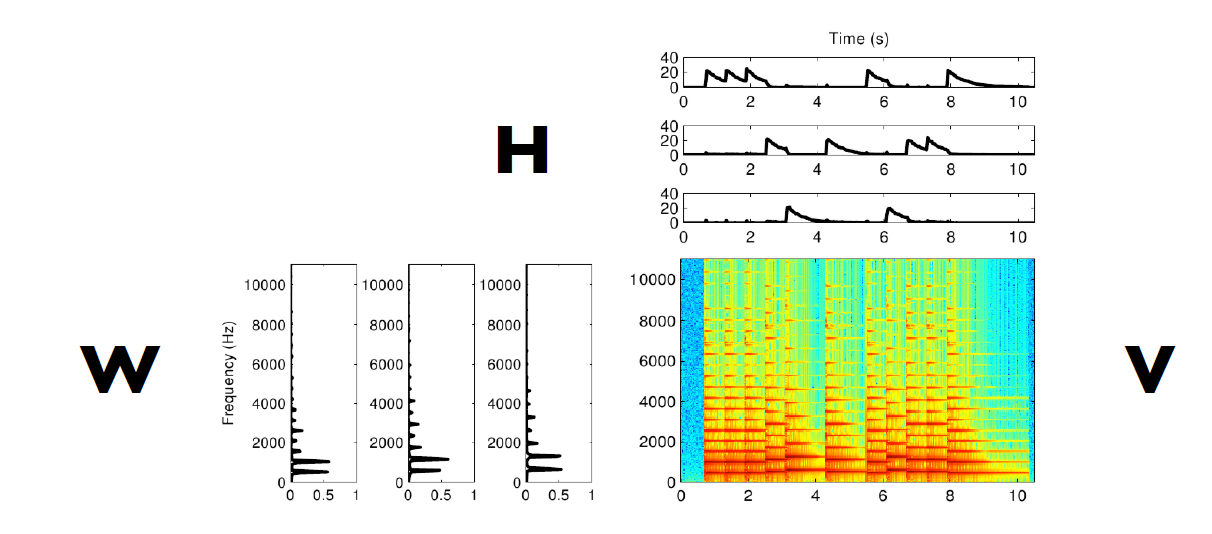
\includegraphics[width=0.9\linewidth]{../image/illustration_NMF.PNG}
\caption{Example of a simple NMF  for a musical content \cite{bertin_les_2009}}
\label{fig:example_NMF}
\end{figure}

The choice of the dimensions is done in a such way that $F\times K + K \times N < F \times N$. To estimate the quality of the approximation, an objective function is used 

\begin{equation}\label{eq:min-D-WH}
\min D\left(\mathbf{V} \vert \vert \mathbf{\tilde{V}}\right) \quad  \textrm{w.r.t.} \quad \mathbf{H} \geq 0, \mathbf{W} \geq 0
\end{equation}

The operator $D(x\vert y)$ is a divergence calculation such as 
\begin{equation}
D\left(\textbf{V} \vert\vert \mathbf{\tilde{V}} \right) = \sum_{f = 1}^{F} \sum_{n = 1}^{N} d_{\beta} 
\left(\textbf{V}_{fn} \vert \left[ \textbf{WH} \right]_{fn} \right)
\end{equation} 

and usually belongs to the $\beta-$divergence class \cite{fevotte_nonnegative_2009} in which the well known Euclidean distance (eq. \ref{eq:def_distEUC}) and the Kullback-Leibler divergence (eq. \ref{eq:def_divKL}) belong

\begin{subequations}\label{eq:divBetaGenerale}
\begin{numcases}{d_{\beta}(x\vert y) =}
    \frac{1}{2}(x-y)^2, & $\beta = 2$, \label{eq:def_distEUC}\\
    x\log \dfrac{x}{y} - x + y, & $\beta = 1$.\label{eq:def_divKL}
\end{numcases}
\end{subequations}

The prior knowledges on the content can be adjust with the add of constraints (like the smoothness or the sparsness criteria \cite{virtanen_monaural_2007}) in the objective function \ref{eq:min-D-WH}. 

NMF can be employed in an unsupervised case where nor $\mathbf{W}$ or $\mathbf{H}$ is known. The \textit{dictionary} is learned first during the training phase with different sound samples, the \textit{basis} got are not retained. $\mathbf{W}$ is afterwards used on the test phase where a new \textit{basis} is got. For the supervised case, $\mathbf{W}$ is already known. In the urban environments, a lot of different sound sources present in the cities are known and their spectrum can be obtained. 
Multiple methods exist to solve the minimization problem (\ref{eq:min-D-WH}) (Alternating Least Square Method \cite{cichocki_regularized_2007}, Projected Gradient \cite{lin_projected_2007} \dots). Here, the multiplicative update is the chosen method \cite{lee_algorithms_2000} as it assures to have a non-negative results where the convergence of the results have been proved \cite{fevotte_algorithms_2011}. The minimization problem (\ref{eq:min-D-WH}) is solved iteratively. As it is the supervised method that is consider first, only the $\mathbf{H}$ is updated. In the first iteration, $\mathbf{H}$ is initialized randomly, then it is updated by the generic  algorithm 

\begin{equation}
\textbf{H}^{(i+1)} \leftarrow \textbf{H}^{(i)}.\left(\frac{\textbf{W}^T \left[\left(\textbf{WH}^{(i)} \right)^{(\beta-2)}.\textbf{V} \right]}{\textbf{W}^T \left[\textbf{WH}^{(i)} \right]^{(\beta-1)}}\right)^{\gamma(\beta)}
\end{equation}

with $\gamma(\beta) = \frac{1}{2-\beta},$ for $\beta < 1$, $ \gamma(\beta) = 1$, for $\beta \in \left[1,2\right]$ and $\gamma(\beta) = \frac{1}{\beta-1}$ for $\beta > 2$. The product $A.B$ and $A/B$ symbolized the Hadamard product.

The source separation is made after $I$ iterations by generating a filtering mask, $M_s$, 
 
\begin{equation} \label{eq:definitionMask}
\mathbf{M_s} = \frac{\left[\mathbf{W} \mathbf{H}\right]_{traffic}}{\sum_{k = 1}^K\left[\mathbf{W H}\right]}, 
\end{equation}

which allows to determine the spectrogram of the traffic component, $ \mathbf{\tilde{V}}_{traffic}$

\begin{equation}\label{eq:separation}
\mathbf{\tilde{V}}_{traffic} = \mathbf{M_s}.\mathbf{V}.
\end{equation}

For the environmental sounds, the method has been used for geo-localisation and classification of the sound environment like in \cite{kumar_audio_2016} where NMF allows to classify the audio files according to the 10 cities where they have been recorded. For the source separation, it has been used by Innami and Kasai in the unsupervised case. They proposed a source separation in two step  by separating the sound background from the events first and by separating the events between them. They used the MFCC features to composed the dictionary by adding a time variant gain features (a calculation of variance and a ratio to nearly zero values on the \textit{basis} vectors). The audio files tested results of a simulation process where a sound background (river or wind) are adding to two sound events (school chime, announcement, frog croaking, dog barging and bell ringing). If the method proposed is interesting, the main issue here is the small size of the database (only 9 sounds) on which the algorithms are tested while some sounds (frog and river) are not representative of sounds that can be found in cities.

\subsection{NMF Semi-supervised}

One of the main issue with the supervised approach is this is not always adapted to different sound environments. Because in the supervised case, the fixed dictionary has to sum up all the sound sources present in the different sound environment. In consequence, as the dictionary dimension is limited and cannot include all the urban sounds, to offer more flexibility, semi-supervised NMF has been proposed \cite{lee_semi-supervised_2010}. This method consists in composing the dictionary $\mathbf{W}_{F \times K+J}$ with a fixed part $\mathbf{W_s}_{F \times K}$ (composed here of traffic audio spectrum) and with a mobile part, $\mathbf{W_r}_{F \times J}$ that is updated. The aim is to include in $\mathbf{W_r}$ the element that are not related with the traffic. The problem (\ref{eq:nmf}) become

\begin{equation}
\mathbf{V} \approx \mathbf{W_s H_s}+ \mathbf{W_r H_r}
\end{equation}

In a similar way as to solve the equation \ref{eq:min-D-WH}, $\mathbf{W_r}$, $\mathbf{H_r}$ and $\mathbf{H_s}$ are successively updated with the relations (\ref{eq:WH-SSupdate}): 

{\scriptsize
\begin{subequations}\label{eq:WH-SSupdate}
\begin{align}
\mathbf{W_r}^{(i+1)} &\leftarrow \mathbf{W_r}^{(i)}.\left(\frac{\left[\left(\mathbf{W_r H_r}^{(i)} \right)^{(\beta-2)}.\mathbf{V} \right]\mathbf{H_r}^T}{\left(\mathbf{W_r H_r}^{(i)} \right)^{(\beta-1)}\mathbf{H_r}^T}\right)^{\gamma(\beta)}\label{eq:W_r_SS}\\
\mathbf{H_r}^{(i+1)} &\leftarrow \mathbf{H_r}^{(i)}.\left(\frac{\mathbf{W_r}^T \left[\left(\mathbf{W_r H_r}^{(i)} \right)^{(\beta-2)}.\mathbf{V} \right]}{\mathbf{W_r}^T \left(\mathbf{W_r H_r}^{(i)} \right)^{(\beta-1)}}\right)^{\gamma(\beta)}\label{eq:H_r_SS}\\
\mathbf{H_s}^{(i+1)} &\leftarrow \mathbf{H_s}^{(i)}.\left(\frac{\mathbf{W_s}^T \left[\left(\mathbf{W_s H_s}^{(i)} \right)^{(\beta-2)}.\mathbf{V} \right]}{\mathbf{W_s}^T \left(\mathbf{W_s H_s}^{(i)} \right)^{(\beta-1)}}\right)^{\gamma(\beta)}\label{eq:H_s_SS}
\end{align}
\end{subequations}}

This approach has been used TO COMPLETE.

\section{Experimental protocol}\label{part:protocol}

NMF are not tested on urban sound recordings: the traffic component is here unknown. Therefore, the estimation of the traffic sound level cannot be compare. In consequence, NMF is applied on simulated sound mixtures as it offers a controlled framework where the contribution of each sound source (and especially the traffic) is known and offers an exact solution to compare with the estimated one.

\subsection{Environmental sound scene corpus}

A first corpus is design with the \textit{simScene} software\footnote{Open-source project available at: \url{https://bitbucket.org/mlagrange/simscene}}. \textit{simScene} \cite{rossignol_simscene:_2015} is a simulator that creates sound mixtures in a .wav format by superposing audio samples that come from an isolated sound database. This database is divided in two categories: the \textit{event} category  which are the brief sounds (from 1 to 20 seconds) that are considered as salient whereas all the sounds that are of long duration and whose acoustic properties do not vary with respect to time belong to the \textit{background} category. Inside each category, the sound samples are grouped in sound classes (\textit{bird, car, foot steps} \dots), each of them being composed of multiples samples (bird01.wav, bird02.wav \dots).

The software allows the user to control some parameters as the number of events of each class that appears in the mixture, the elapsed time between each sample of a same class or the presence of a fade in and a fade out \dots. Each parameter is completed with a standard deviation that may brings some random behavior between the scenes. Furthermore, with the global scene mixture, an audio for each sound class presented in the scene can be generated that allow to know its exact contribution and a text file is created that sum up the time presence of all the event.\\

\begin{figure}[h]
\centering
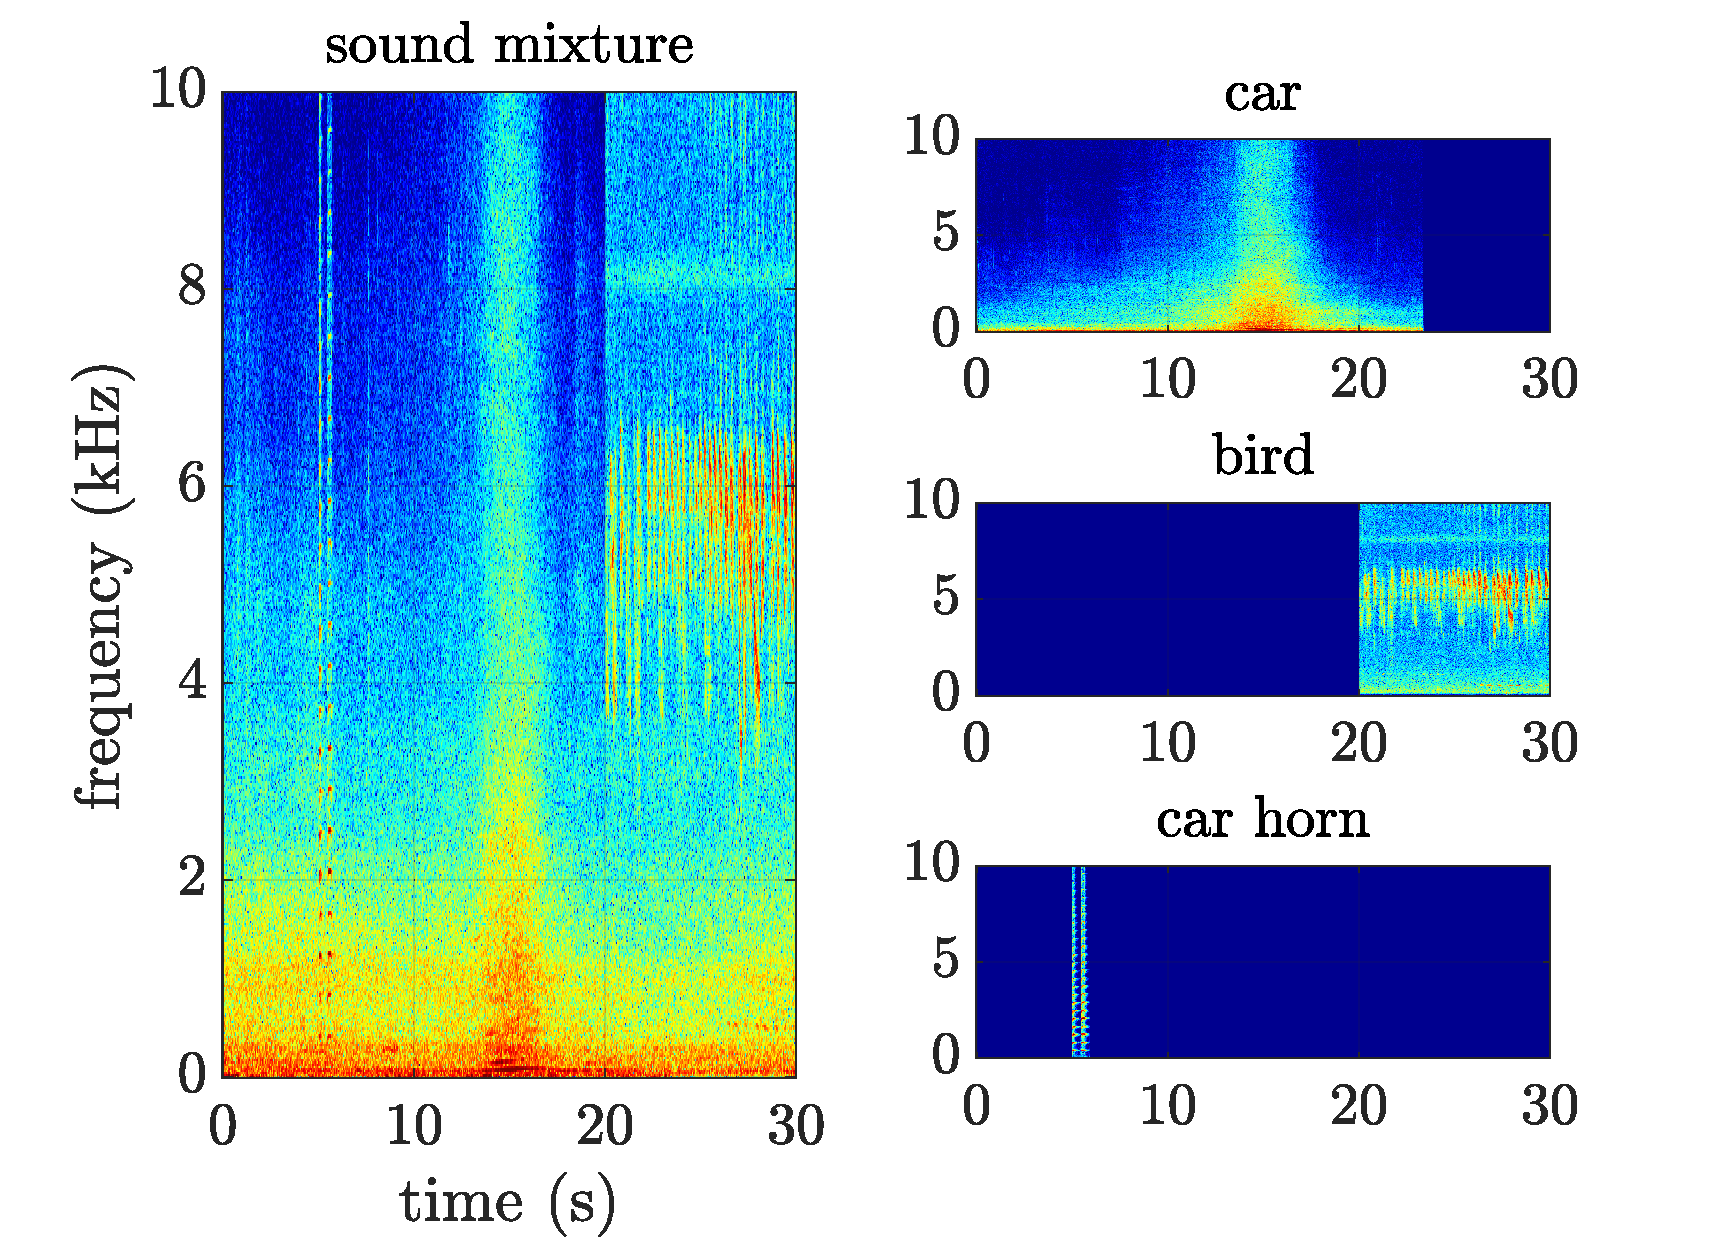
\includegraphics[width=\linewidth]{../image/exampleSimScene.pdf} 
\label{fig:exampleSimScene}
\caption{Example of a sound mixture composed of 3 sound classes (car, bird, car horn)}
\end{figure}

With this software, a sound database has been built including 245 sound event samples (with the sound classes \textit{ringing bell, birds, sweeping bropom, car horn, car passages, hammer, drill, coughing, barking dog, rolling suitcase, closing door, plane, siren, footstep, storm, street noise, train, tramway, truck and voice}) and 154 sound background samples (\textit{birds, construction site noise, crowd, park, rain, children playing in schoolyard, constant traffci noise, ventilation, wind}). The sound class \textit{car passages} comes from recordings of 4 cars made on the Ifsttar's runway  on different speeds with multiple gear ratio \cite{gloaguen_creation_2017}. The other audio files are sampled at 44.1 kHz and have been found online (\textit{freesound.org}) and with the help of the \textit{UrbanSound8k} database \cite{salamon_dataset_nodate}. A sound mixture corpus is designed composed of 6 sub-corpus of 25 30 seconds audio files ($N = 25$). Each sub-corpus is characterized by a specific generic sound class : \textit{alert} (car horn, siren), \textit{animals} (barking dog , whistling birds), \textit{climate} (wind, rain), \textit{humans} (crowd noise and voice), \textit{mechanics} (different metallic and construction site noise) and \textit{transportation} (train, tramway and plane). In each file, traffic component is present as sound background and event and is mixed with on or multiple sound classes. The sound classes that are not related to the traffic component are summed up as the \textit{perturbator} (n'existe pas comme terme, disruptive ?) class. To test different scenarios, each audio file is duplicated with the traffic sound level of the entire sound mixture, $L_{p,traffic}$, fixed to a specific level according to the sound level of the \textit{perturbator} class, $L_{p,perturbator}$ following the relation (\ref{eq:tpr}). 

\begin{equation}\label{eq:tpr}
TPR = L_{p,traffic}-L_{p,perturbator}
\end{equation}

with the \textit{Traffic Perturbator Ratio} $TPR = \left[-12, -6, 0, 6, 12\right]$. When $TPR = -12$, the traffic component is then less present than when $TPR = 12$ where it is predominant on the \textit{perturbator} class. The 1 second equivalent sound pressure level, $p_{1s,traffic}$, is too calculated (figure \ref{fig:exampleScene}). Finally, the number of scenes designed is 750 (6 sub-corpus $\times$ 25 scenes $\times$  5 TPR values). 

\begin{figure*}
\centering
   \begin{minipage}[c]{.32\linewidth}
      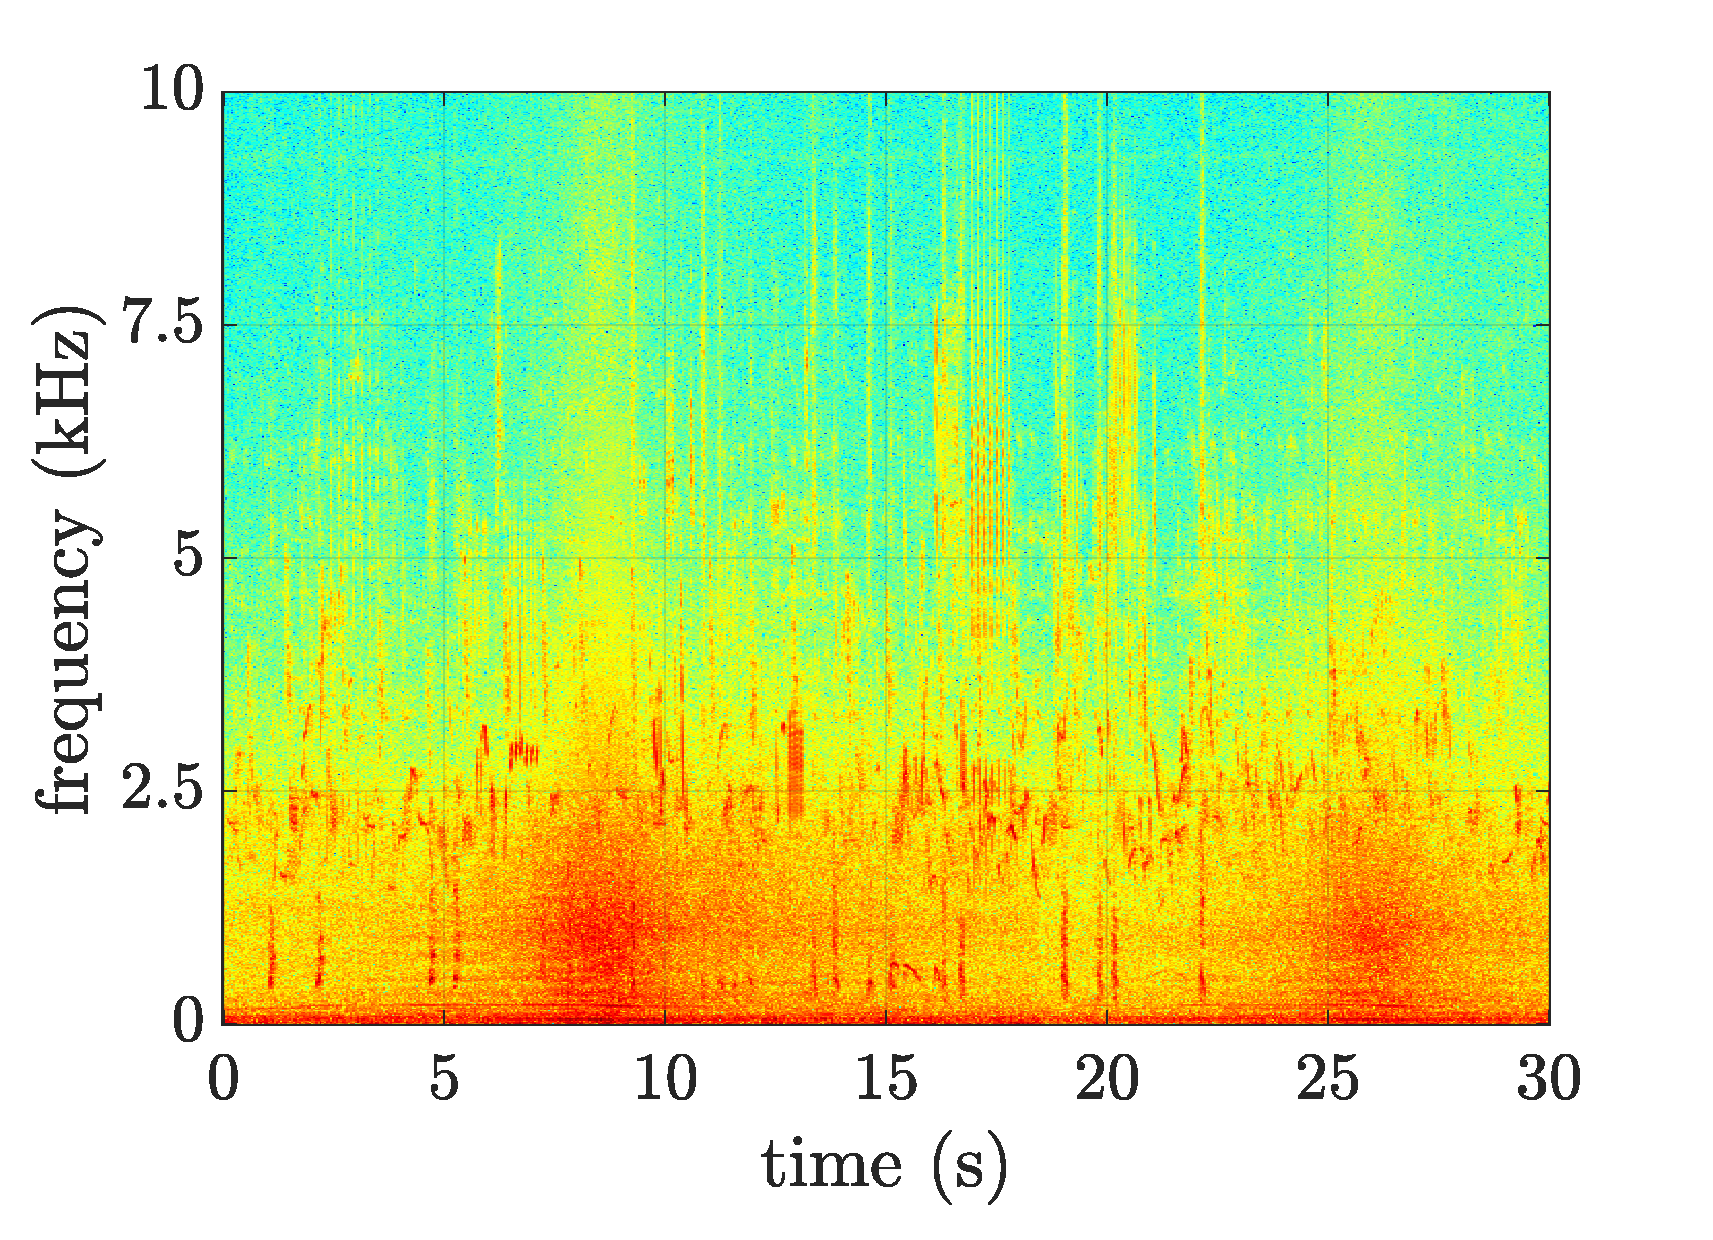
\includegraphics[width =\linewidth]{../image/spectrogramExample.pdf} 
   \end{minipage} 
   \begin{minipage}[c]{.32\linewidth}
      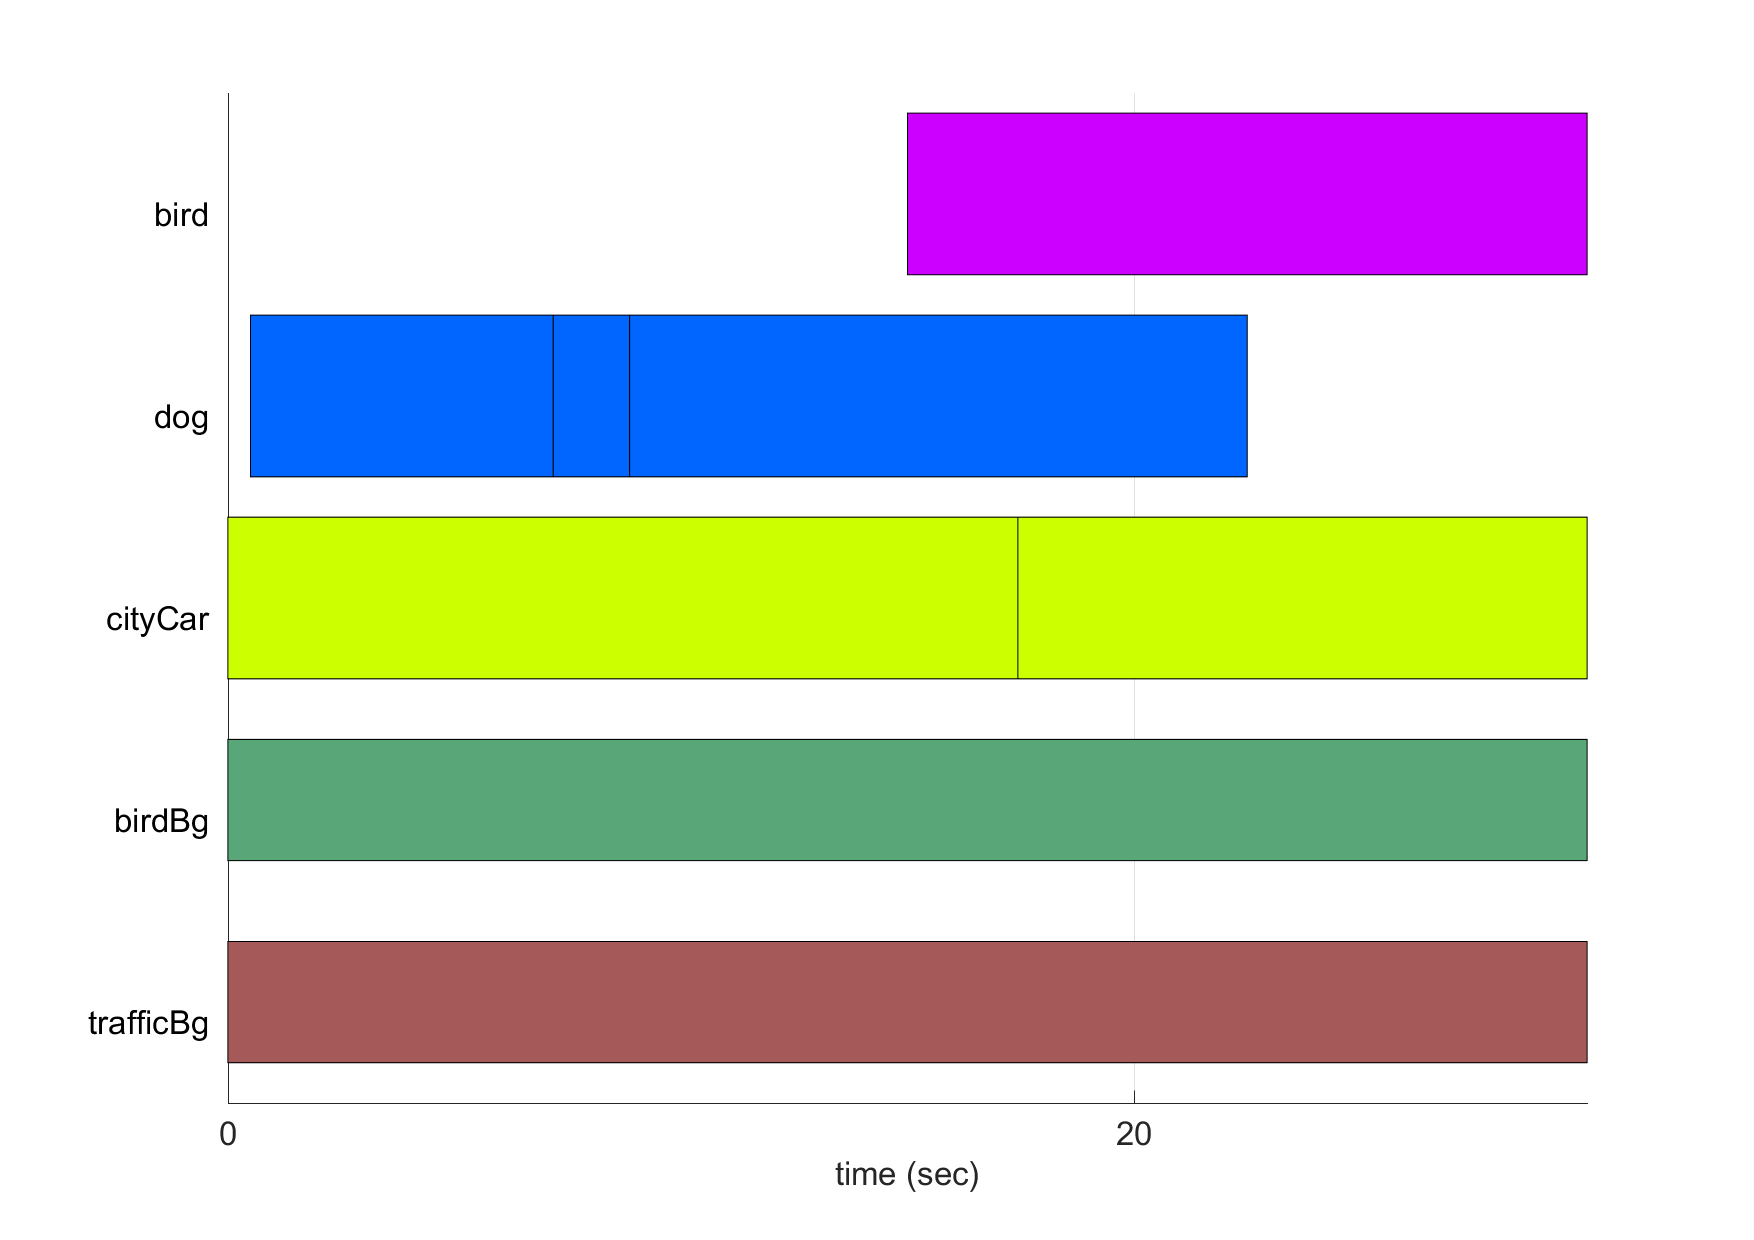
\includegraphics[width =\linewidth]{../image/animals_10-pianoRoll.png} 
   \end{minipage} 
   \begin{minipage}[c]{.32\linewidth}
      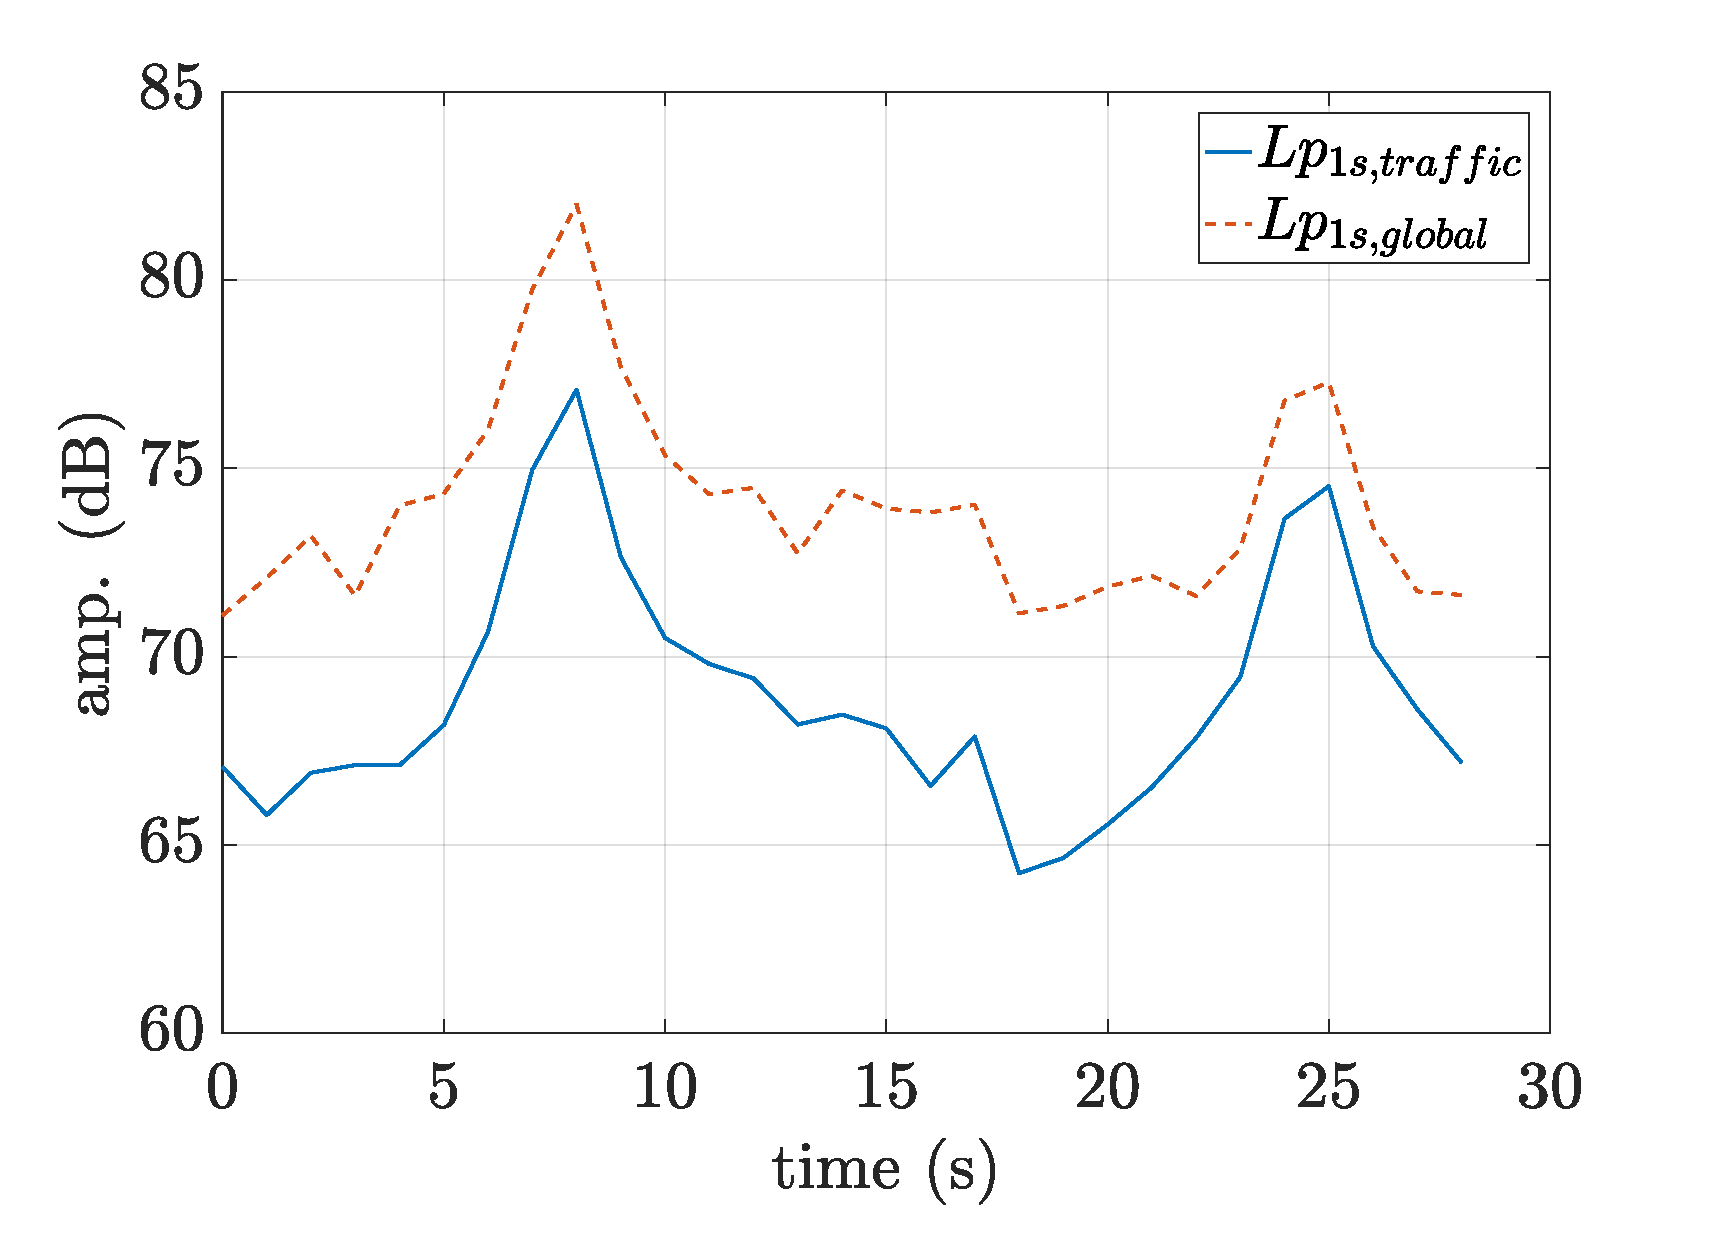
\includegraphics[width =\linewidth]{../image/evolutionLpExample.pdf} 

   \end{minipage}
\caption{Example of a scene of the \textit{animals} sub corpus. Spectrogram (on left), \textit{Piano Roll} of the different sound classes (on the middle) and 1-s equivalent sound level of the traffic, $Lp_{1s,traffic}$ and of the global sound mixture, $Lp_{1s,global}$(on right)}
\label{fig:exampleScene}
\end{figure*}

\subsection{Experiment}

The experiment consists in applied NMF on the environmental sound corpus to estimate the sound level of the traffic road. This method is compared to a simple approach which is a low-frequency filter. This method considers, as the traffic component is mostly composed of low-frequencies, that the sound level can be calculated from the band-pass filter. Similarly, the low-pass filter is applied with NMF with the aim to focus the reconstruction of the signal on the frequencies where the traffic components are. The figure \ref{fig:block_diagram_protocol} sum up the different step of the process depending on the chosen method.\\

\begin{figure*}[!t]
\centering
	\begin{minipage}[t]{.48\textwidth}
		\centering
		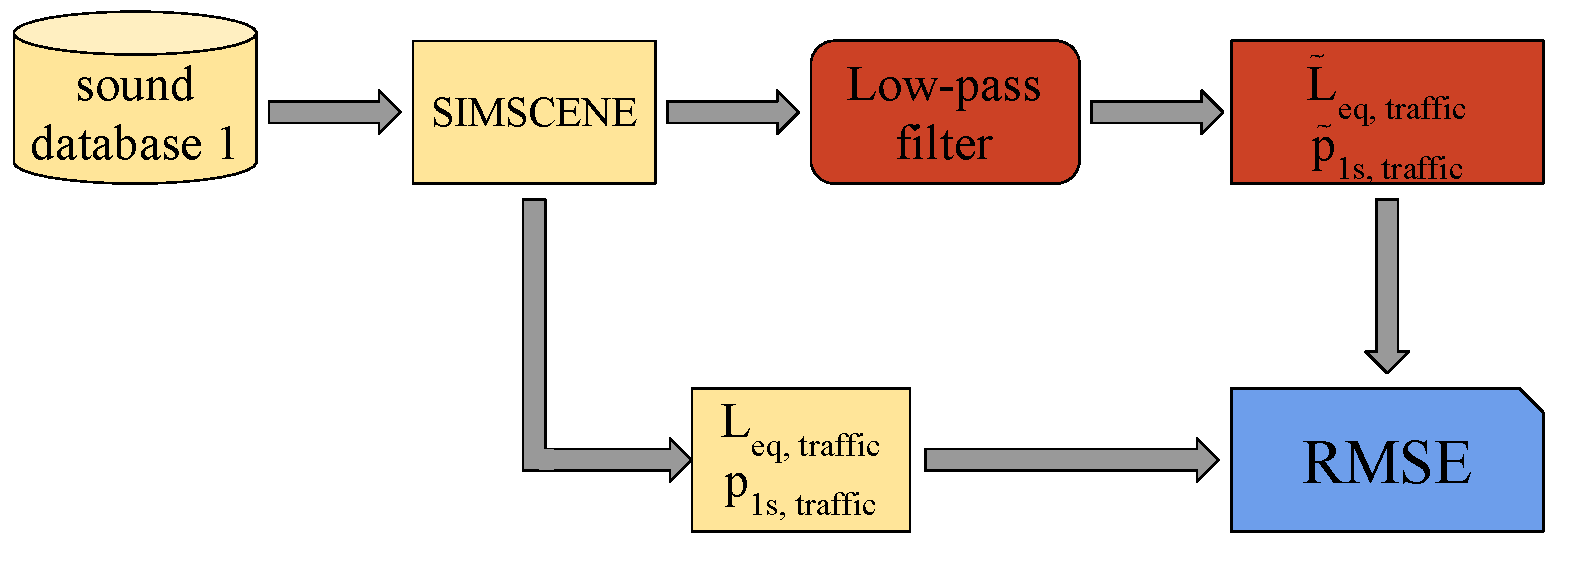
\includegraphics[width=.9\linewidth]{../image/bloc_diagram_filtrage_EN.pdf} 
	\end{minipage}
	\begin{minipage}[t]{.48\textwidth}
		\centering
		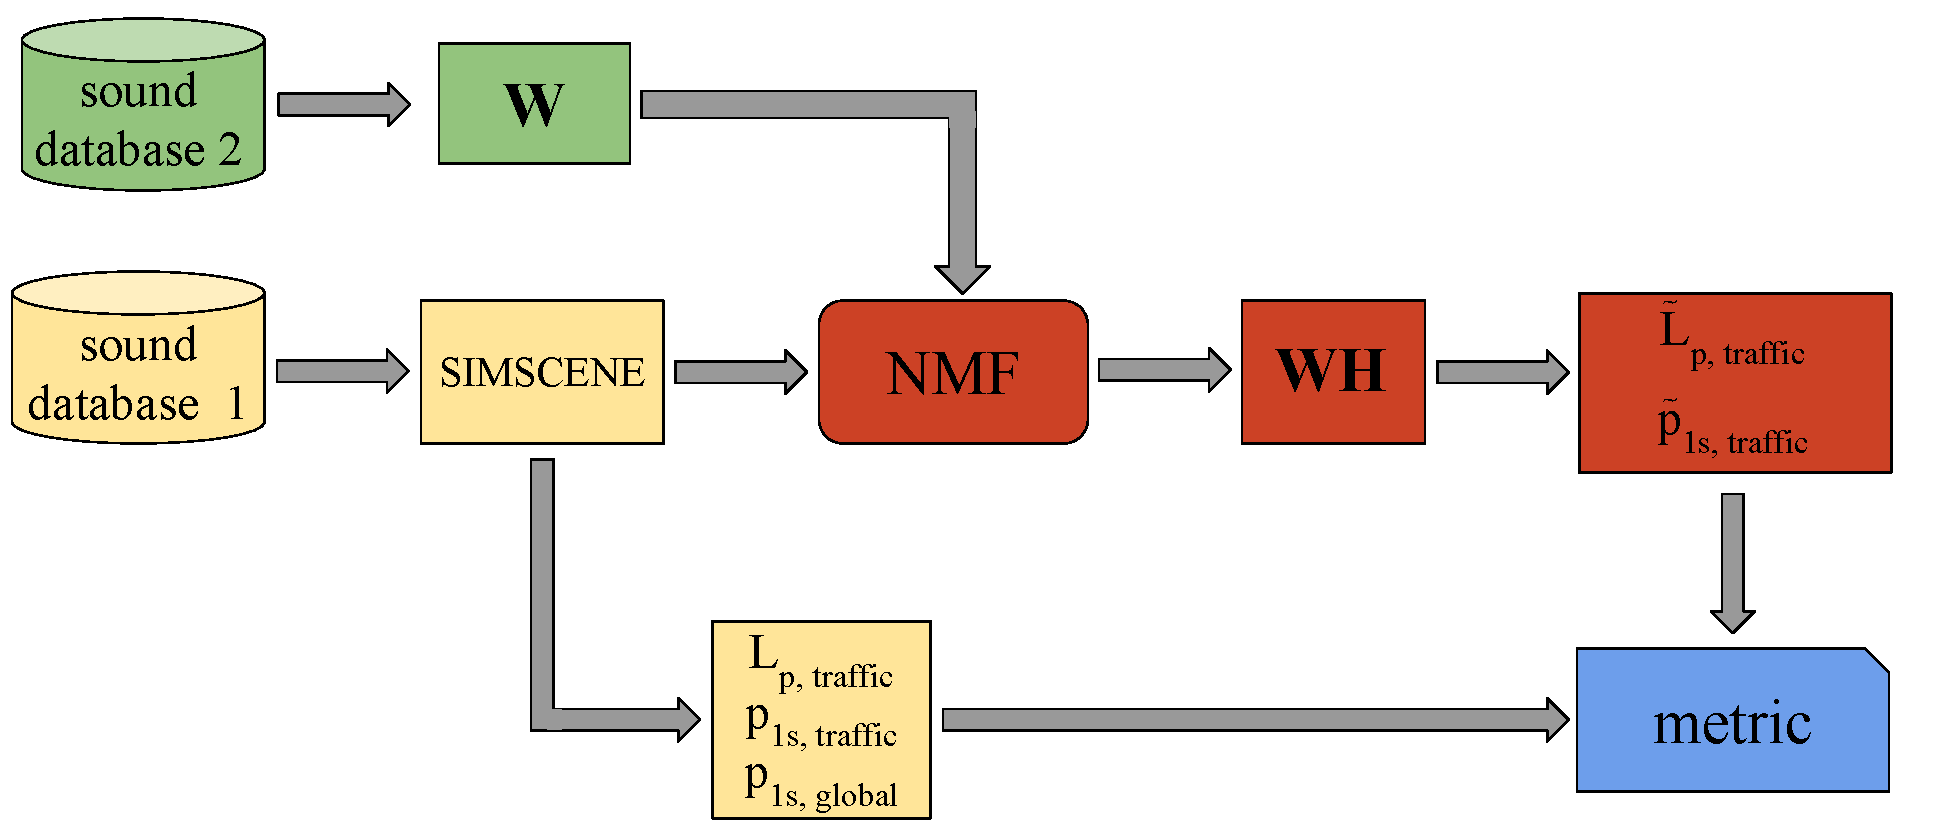
\includegraphics[width=.9\linewidth]{../image/bloc_diagram_NMF_EN.pdf} 
	\end{minipage}
	\caption{Block diagrams summed up the different step of the precess. On top, for the low-pass filter, on bottom, for NMF.}
	\label{fig:block_diagram_protocol}
\end{figure*}

3 calculation steps are set up : 
\begin{itemize}
\item the dictionary building for NMF
\item the estimation of the traffic sound level according the chosen method (NMF or low-pass filter)
\item calculation of the error between the exact and the estimated sound levels.\\
\end{itemize}

\subsubsection{Dictionary building}

The dictionary is built from a sound database dedicated specially to this task. It is composed of 53 audio files of car passages. Multiple version of dictionaries are tested. First, for each audio file, its spectrogram is calculated with fixed parameters ($w = 2^{14}$, $noverlap = 75 \%$, $nfft = 2^{14}$). Then a temporal rectangular window of 0.5 second is applied without overlapping on the spectrogram. In each window, the root mean square value are calculated. This window allow to get multiples spectrum from an audio file.  An example, to illustrate the process, can be found on figure with a large window of 4 seconds. 

\begin{figure}[!t]
\centering
	\begin{minipage}[t]{.24\textwidth}
		\centering
		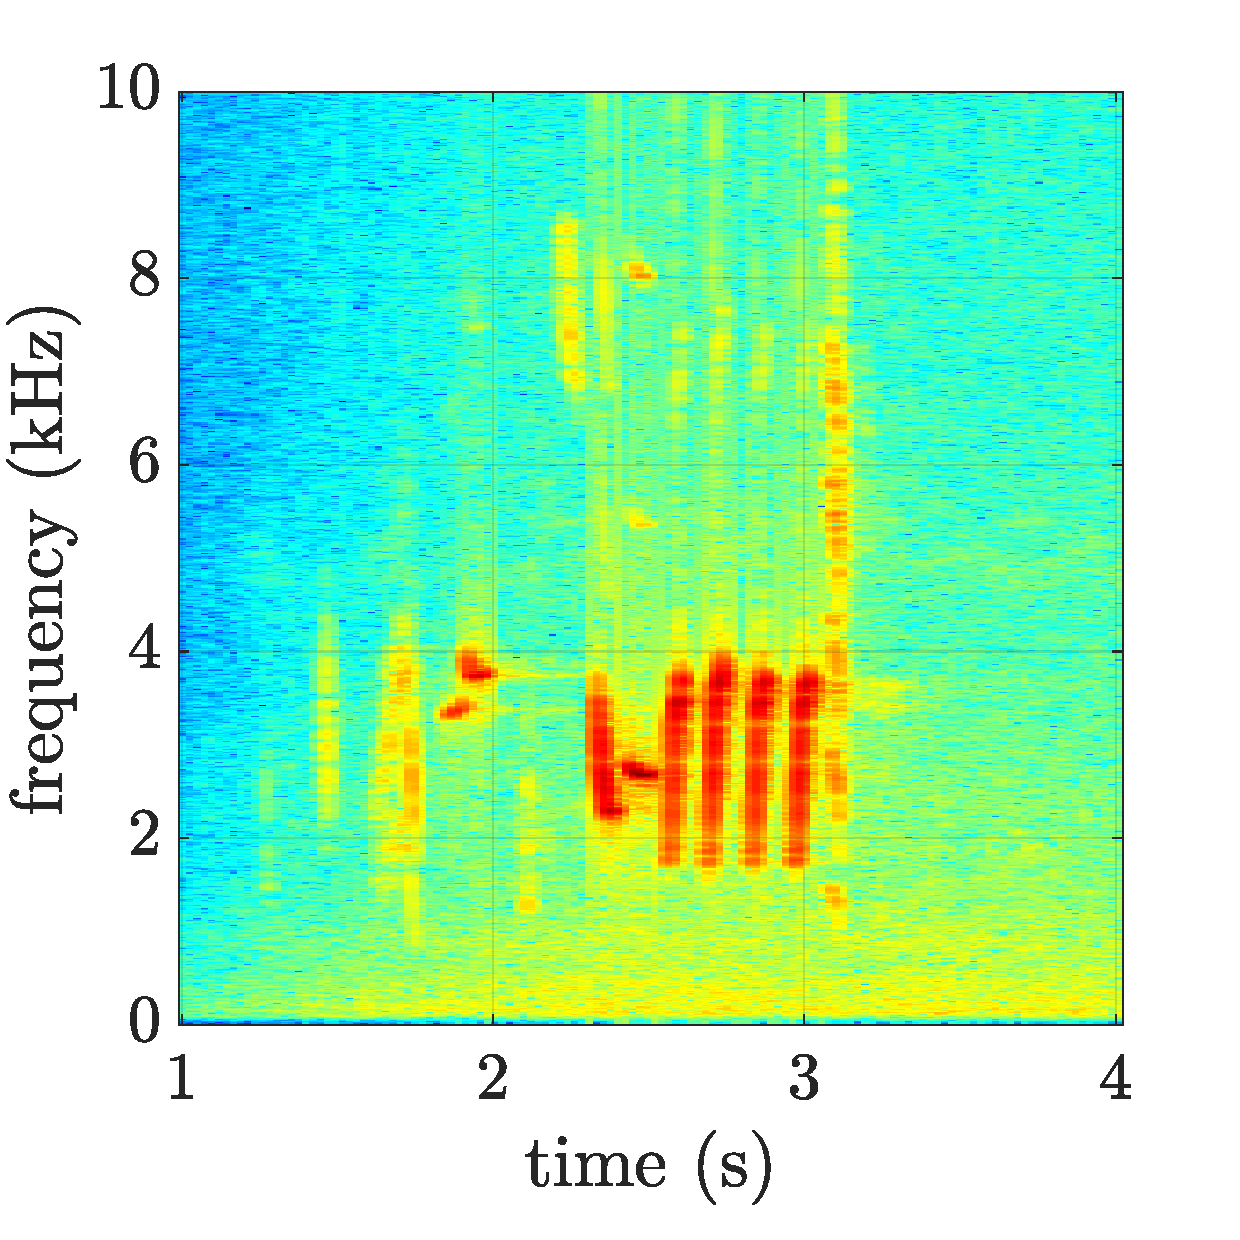
\includegraphics[width=.9\linewidth]{../image/extractionDictionary1Example.pdf} 
	\end{minipage}
	\begin{minipage}[t]{.24\textwidth}
		\centering
		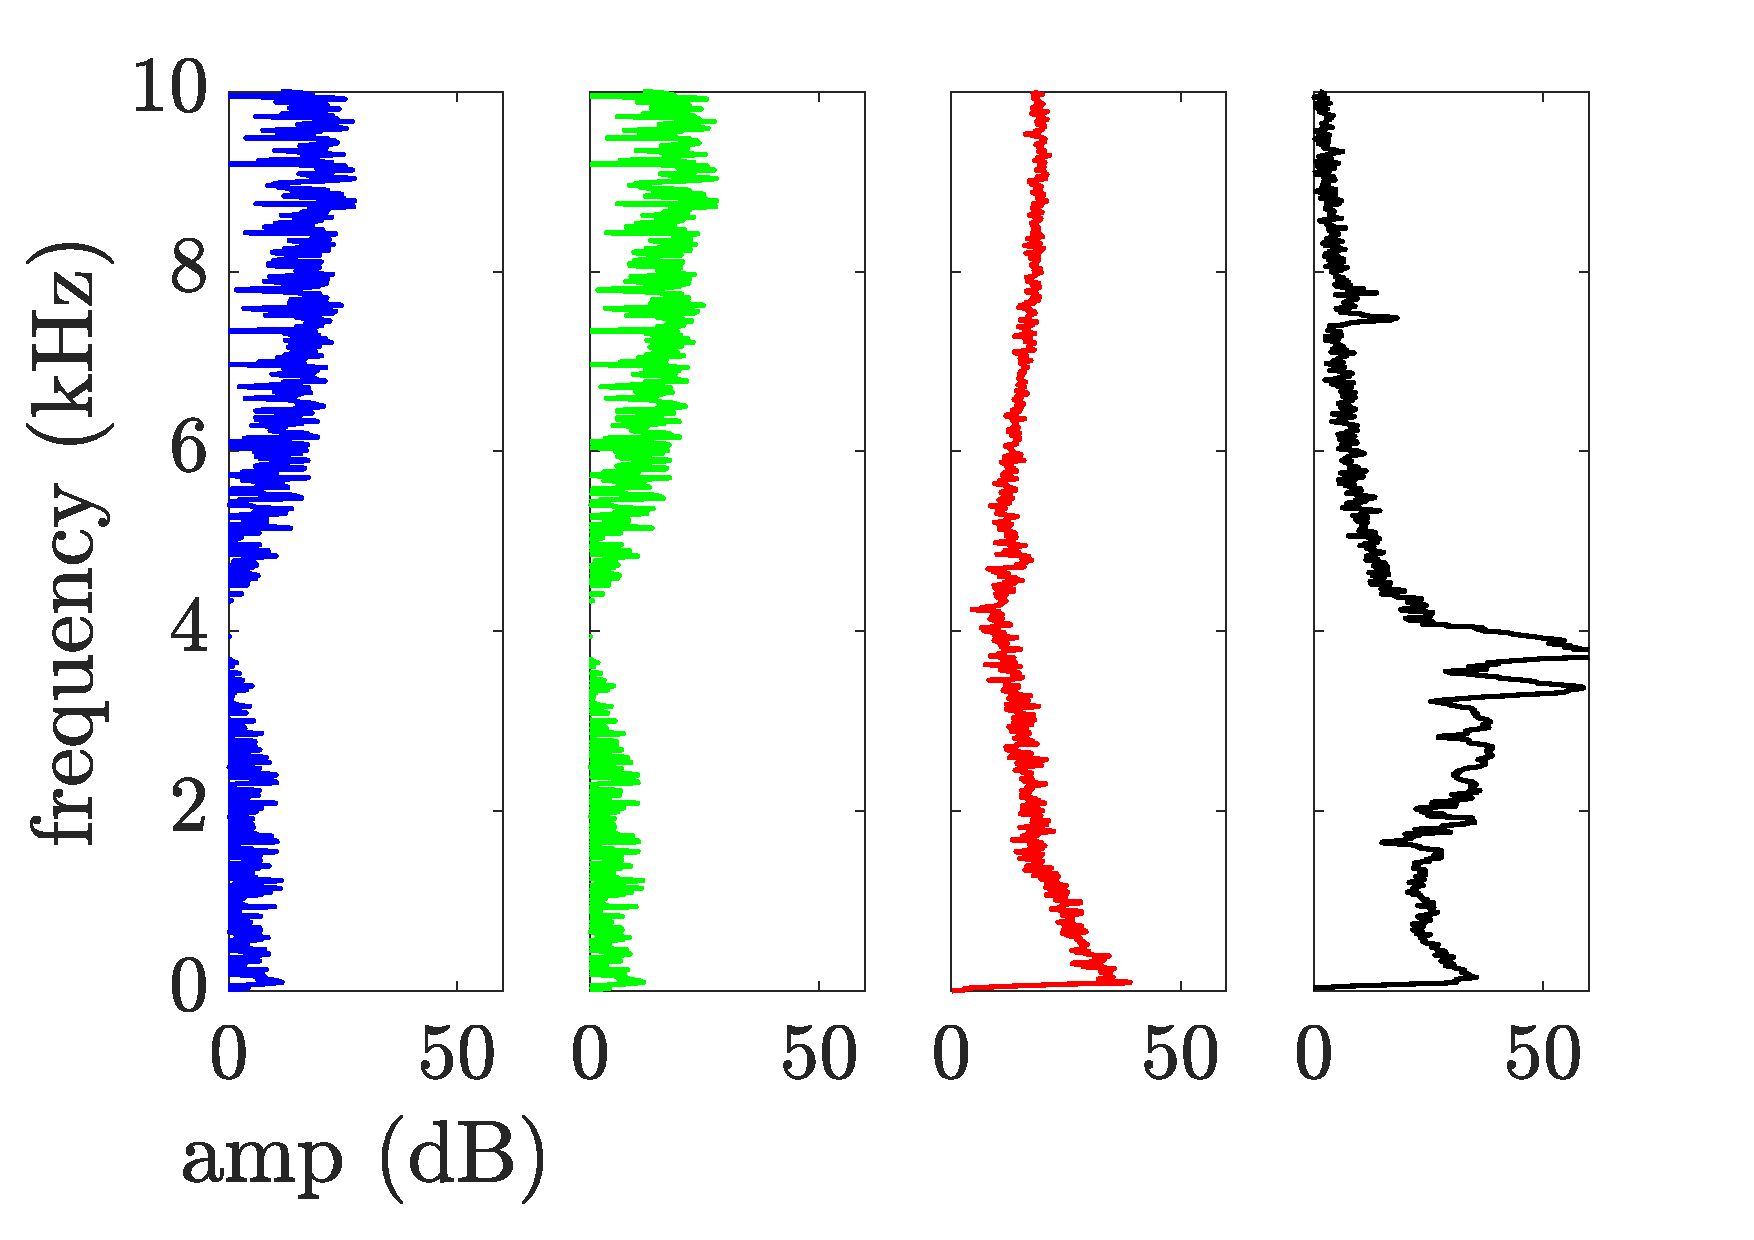
\includegraphics[width=.9\linewidth]{../image/extractionDictionary2Example.pdf} 
	\end{minipage}
	\caption{Example of the extraction of the spectrum with a 4 seconds window. On left, the original spectrogram with the temporal window, on the left, the 4 spectrum obtained (dB scale)}
	\label{fig:dictionaryExtraction}
\end{figure}

As the number of spectrum got on all the sound database does not respect the constraint imposed about the dimension of NMF, a $K$-medoid clustering is applied to reduce the number of spectrum to $K = \left[ 25, 50, 100 \right]$. A special case is added where the root mean square of the spectrum is applied on all the spectrogram. In consequence, the audio file is summed up in one spectra. 
% It consists in the estimation of the $K$-means and then to calculate the euclidean distance between each centroid with all the spectrum. The spectrum having the smaller distance with the centroid is then included in the dictionary $\mathbf{W}$.

\subsubsection{Estimation of the traffic sound level}
\subsubsection{Low-pass filter}
The first estimator to determine the traffic sound level is a basic low-pass filter with the cut-off frequencies $f_c = \left[ 500, 1k, 2k, 5k, 10k, 20k\right]$ Hz. As the road traffic is mainly composed of low frequencies (< 5000 Hz), this method considers that all the components located on the pass-band can be considered as road traffic. 
\subsubsection{NMF}
The second estimator is NMF with the supervised and the semi-supervised approaches (see part \ref{part:nmf}). The spectrogram $\mathbf{V}$ and the dictionary $\mathbf{W}$ are expressed on two different formats: with a linear frequency scale ($\Delta f \approx 2.8$ Hz) and with third octave bands. Theses two methods enables to compare a fine approach (the linear scale) with a degraded one (the third octave bands) as it reduces the number of frequency bins (27 bands) and allows to reduces the number of bands in the high frequencies where the traffic component is less present. Furthermore, in the case of the linear frequency scale, $\mathbf{V}$ and $\mathbf{W}$ are filtered at the frequencies $f_c$ in order to focused the reconstruction of the signal of the low frequency bins. The $\beta$-divergence is reduced to the Kullback-Leibler divergence ($\beta = 1$) and to the Euclidean distance ($\beta = 2$). 400 iterations are performed. 
The source separation is performed following equations (\ref{eq:definitionMask}) and (\ref{eq:separation}) according two ways: based on the filtered elements ($\mathbf{V}_{f_c}$ and $\mathbf{W}_{f_c}$) or on the entire spectrogram and dictionary ($\mathbf{V}$ and $\mathbf{W}$). Then for each spectrogram, the estimated equivalent traffic sound level in dB of the entire scene, $\tilde{L}_{p,traffic}$, is calculated as well as the 1 second equivalent sound pressure level, $\tilde{p}_{1s,traffic}$. 

\subsubsection{Metric}
The performances of the two estimators to estimate the sound level of the traffic correctly are estimated through the calculation of two metrics based on the Root Mean Square Error (RMSE) : 

\begin{itemize}
\item the global RMSE, \textit{gRMSE}, which consists in calculate for each combination of factors the error between the exact and estimated global traffic sound level in dB of the $N$ scenes.

\begin{equation}
gRMSE = \sqrt{\frac{1}{N}\sum_{n = 1}^N \left(L^n_{p,traffic}-\tilde{L}^n_{p,traffic}\right)^2}
\end{equation}

This metric expresses the quality of the long-term reconstruction of the signal. 
\item The normalized short-term RMSE, $nRMSE$, consists in calculate, for each sound mixture, the error between the 1-s equivalent sound level exact and estimated of the traffic of each file normalized by the 1-s equivalent sound level of the global mixture in the linear scale, 

\begin{equation}
nRMSE = \sqrt{\frac{1}{T}\sum_{t = 1}^T \left(\frac{p^t_{1s,traffic}-\tilde{p}^t_{1s,traffic}}{p^t_{1s,global}}\right)^2}
\end{equation}

with $T$ is the number of temporal bin in the signal. The linear scale is here more relevant than the dB scale as it is more sensitive to the error on the high sound levels. Then for one combination of factors, the $N$ $nRMSE$ calculated are averaged.\\
\end{itemize}
The calculation are performed in 3 steps. The first set up the dictionary with two modalities : $K$ value (25 50 100) and description of the audio files (in one fft or with a temporal window of 0.5 second). The second step include  modalities : the sub-corpus (\textit{alert} (al), \textit{animals} (an), \textit{humans} (hu), \textit{climate} (cl), \textit{mechanics} (me), \textit{transportation} (tr)), the estimator (low-pass filter, NMF), the cut-off frequency $f_c$ ([500 1k 2k 5k 10k 20k] Hz), the $TPR$ ([-12 -6 0 6 12] dB), $\beta = [1~2]$, the approach NMF  (supervised or semi-supervised) and the frequency scale (linear or third octave). In all, 5940 settings are performed.

\section{Results}\label{part:results}

In a first time, the low-pass filter estimator is performed on all the scene. The table \ref{tab:results_filter} sums up the mean error on the totality of the 750 scenes to find the cut-off frequency the most efficient on all the cases. 

\begin{table}[h]
\centering
\begin{tabular}{lll}
$f_c$ (Hz) & $nRMSE$ & $gRMSE$ (dB) \\ \hline
\textbf{500}  &\textbf{1.48 $\pm$ 1.10}&\textbf{5.96 $\pm$ 6.70}\\ \hline
1k &  1.52 $\pm$ 1.34 & 6.52 $\pm$ 7.73\\ \hline
2k & 1.57 $\pm$ 1.54 & 6.80 $\pm$ 8.32\\ \hline
5k & 1.82 $\pm$ 1.65 & 7.44 $\pm$ 8.89       \\ \hline
10k  & 1.89 $\pm$ 1.70 & 7.56 $\pm$ 8.99       \\ \hline
20k  & 1.89 $\pm$ 1.72 & 7.59 $\pm$ 9.02      
\end{tabular}
\caption{RMSE error for the low pass filter averaged on all the TPR and sub-classes}
\label{tab:results_filter}
\end{table}

According the table, the cut-off frequency at 500 Hz is the most efficient on all the TPR and all the sub-classes. The error for a 500 Hz cut-off frequency according to the sub-classes and the TPR is sums up in the figure \ref{fig:filterAmbiance}.

\begin{figure}[hbtp]
\centering
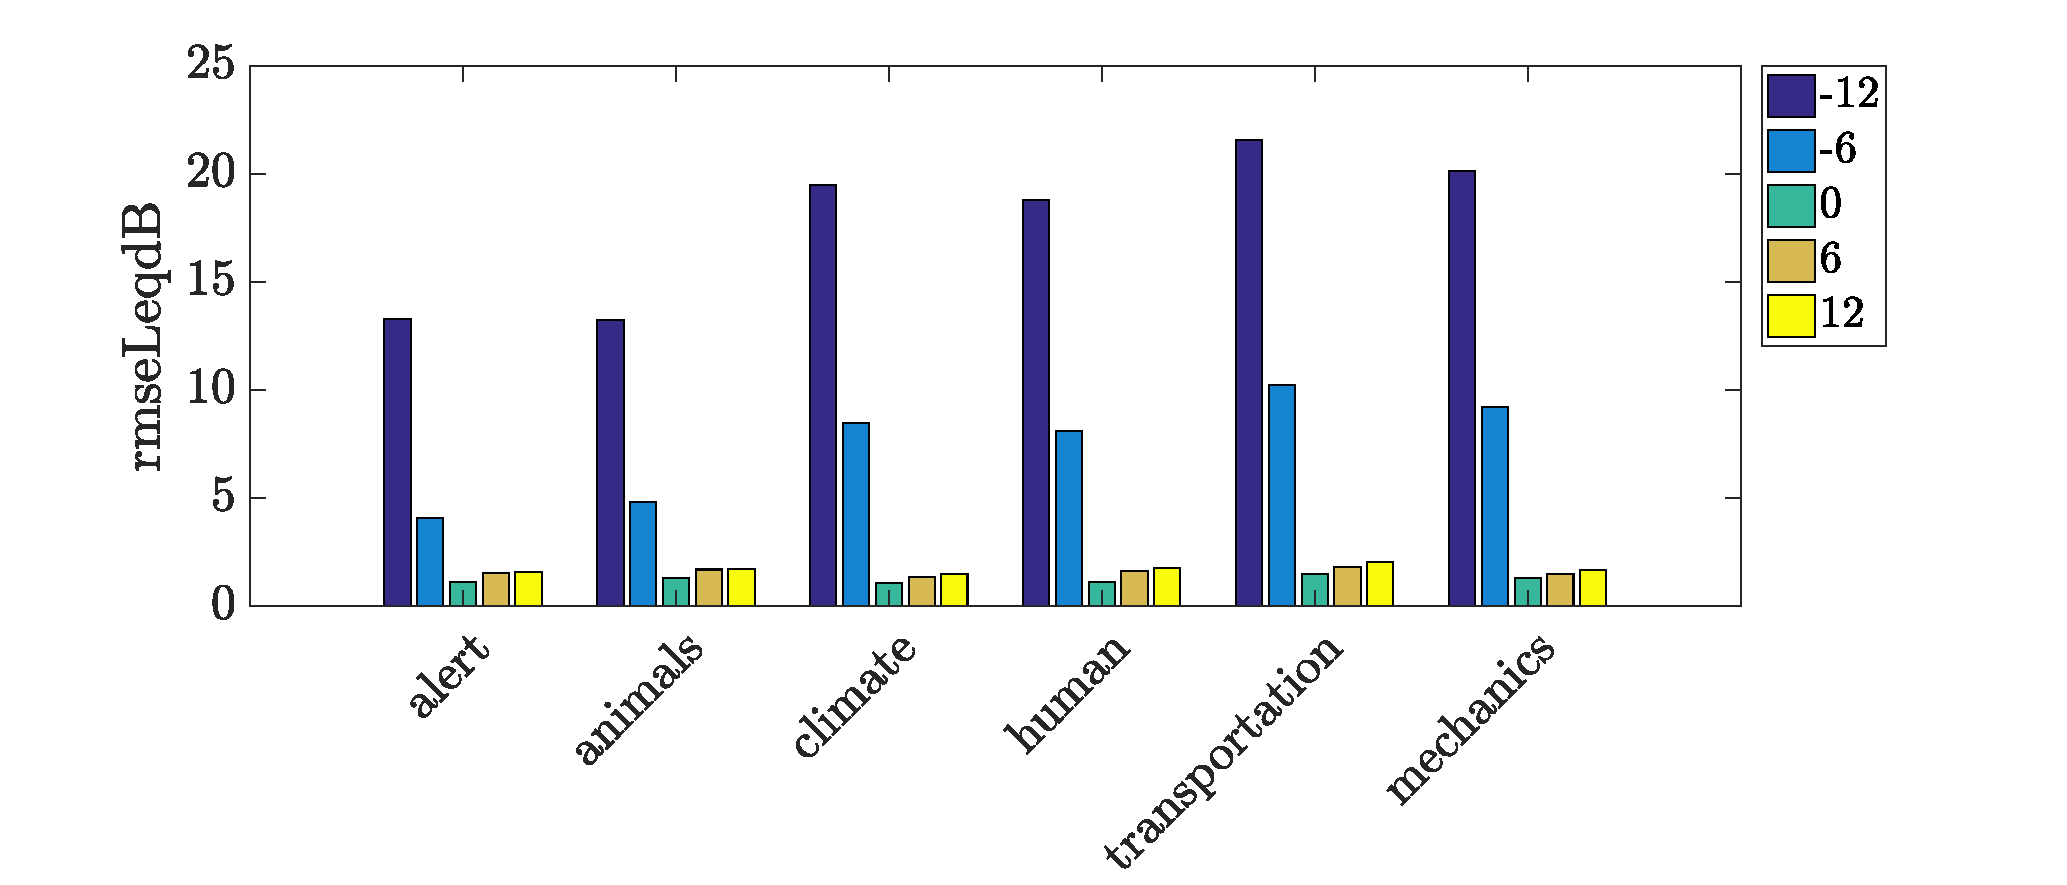
\includegraphics[width=\linewidth]{../image/filterAmbianceBar.pdf}
\caption{Bar plot for the low-pass filter according to the sub-classes and the TPR at 500 Hz cut-off frequency}
\label{fig:filterAmbiance}
\end{figure}

The error for all the sub-corpus is important for the low TPR (-12 and -6) due to the confusion of the \textit{perturbator} class as the traffic component whereas  it is not. The error is less for the \textit{alert} and \textit{humans} sub-corpus as it is composed of higher frequencies while for the \textit{climate} and \textit{transportation} the error is far more important. For the other TPR, the traffic is more present and become dominating on the \textit{perturbator} class. Then the error is due to the suppression of the traffic energy by the low-pass filter. 

The first results averaged on all the TPR and the sub-classes for the supervised NMF is sums up on table \ref{tab:}, the frequency domain is, for now, limited to \textit{spectra}

\begin{table}[h]
\centering
\begin{tabular}{lll}

\end{tabular}
\caption{RMSE error for the low pass filter averaged on all the TPR and sub-classes}
\label{tab:results_filter}
\end{table}


Résultat global pour le NMF supervisée en tableau puis en bar pour chaque ambiance et chaque TPR
Tracer l'évolution 1s du signal sonore pour 2 ambiances et 2 TPR
résultat semi-supervisée
beta = 2, = 1
%

\section{Conclusion}
\footnotesize
\bibliographystyle{unsrt}
\bibliography{bibliographie_applied}

\end{document}